

\section{Results}

\begin{itemize}
  \item \hl{style change on the fly performance (time per frame)}
  \item \hl{generate high resolution style transfer + save+send image performance (seconds)}
\end{itemize}

\subsection{Preprocessing: face and emotion detection}

\begin{figure}[ht]
    \centering
        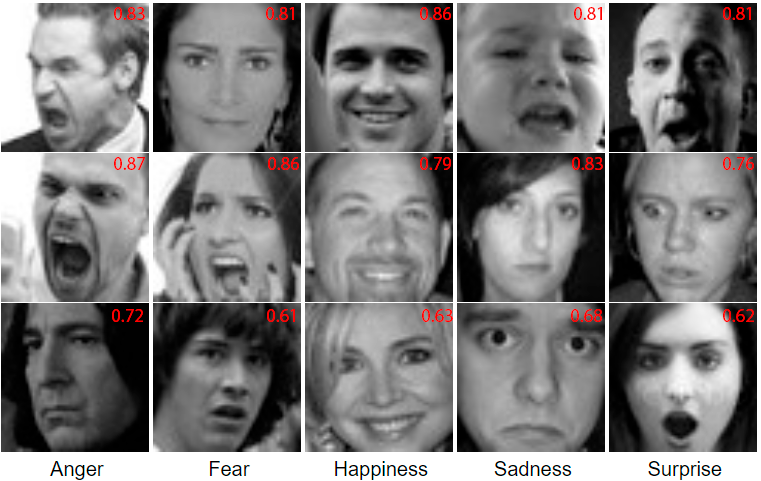
\includegraphics[width = 9cm]{resources/emotion_faces_1.png}
         \label{fig:emotion_faces}
\end{figure}
  

\begin{figure}[h]
    \centering
       \begin{subfigure}{0.49\linewidth} \centering
         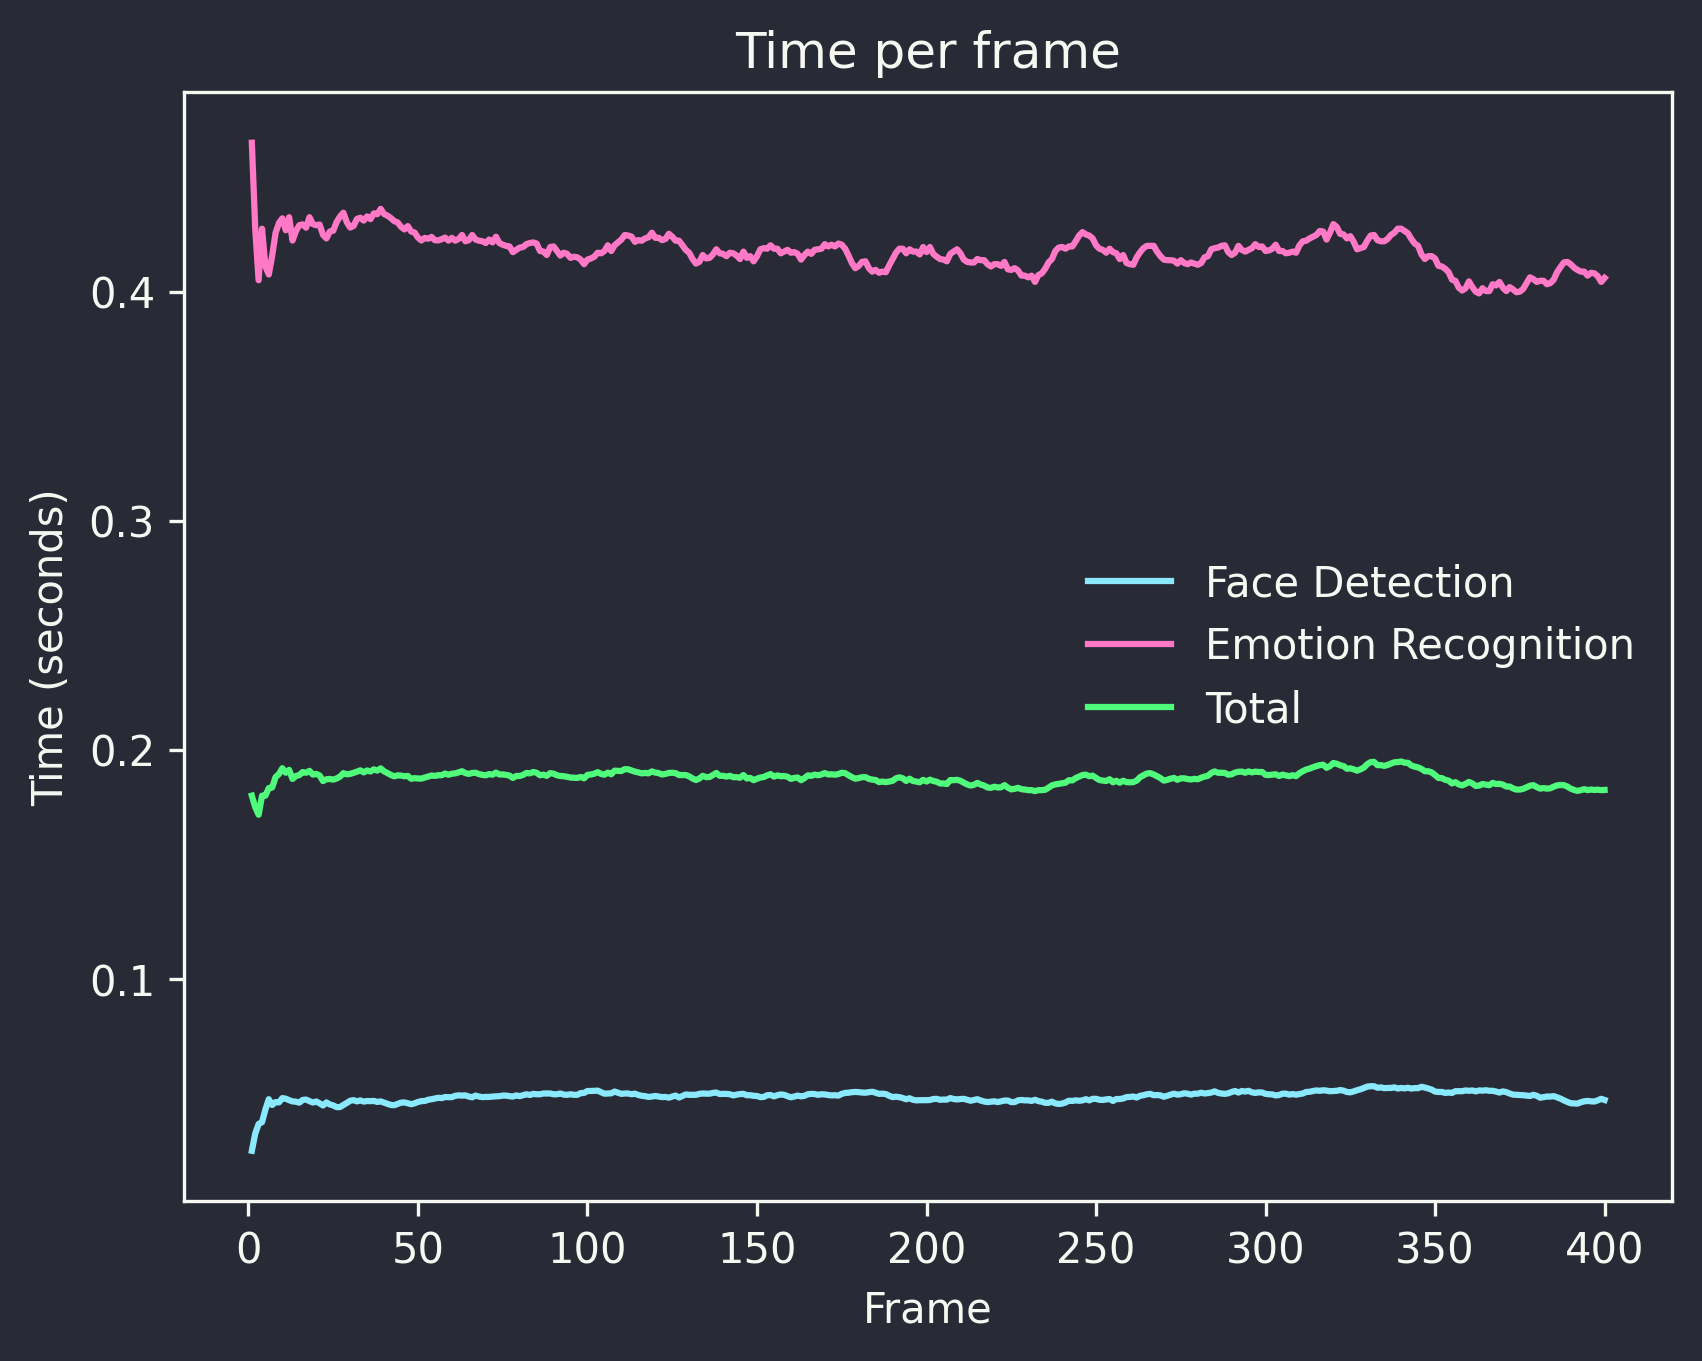
\includegraphics[height = 6cm]{resources/face_emo_time_series.png}
         \caption{Time needed to process a frame.}\label{fig:timeseriesplot}
       \end{subfigure}
       \begin{subfigure}{0.49\linewidth} \centering
         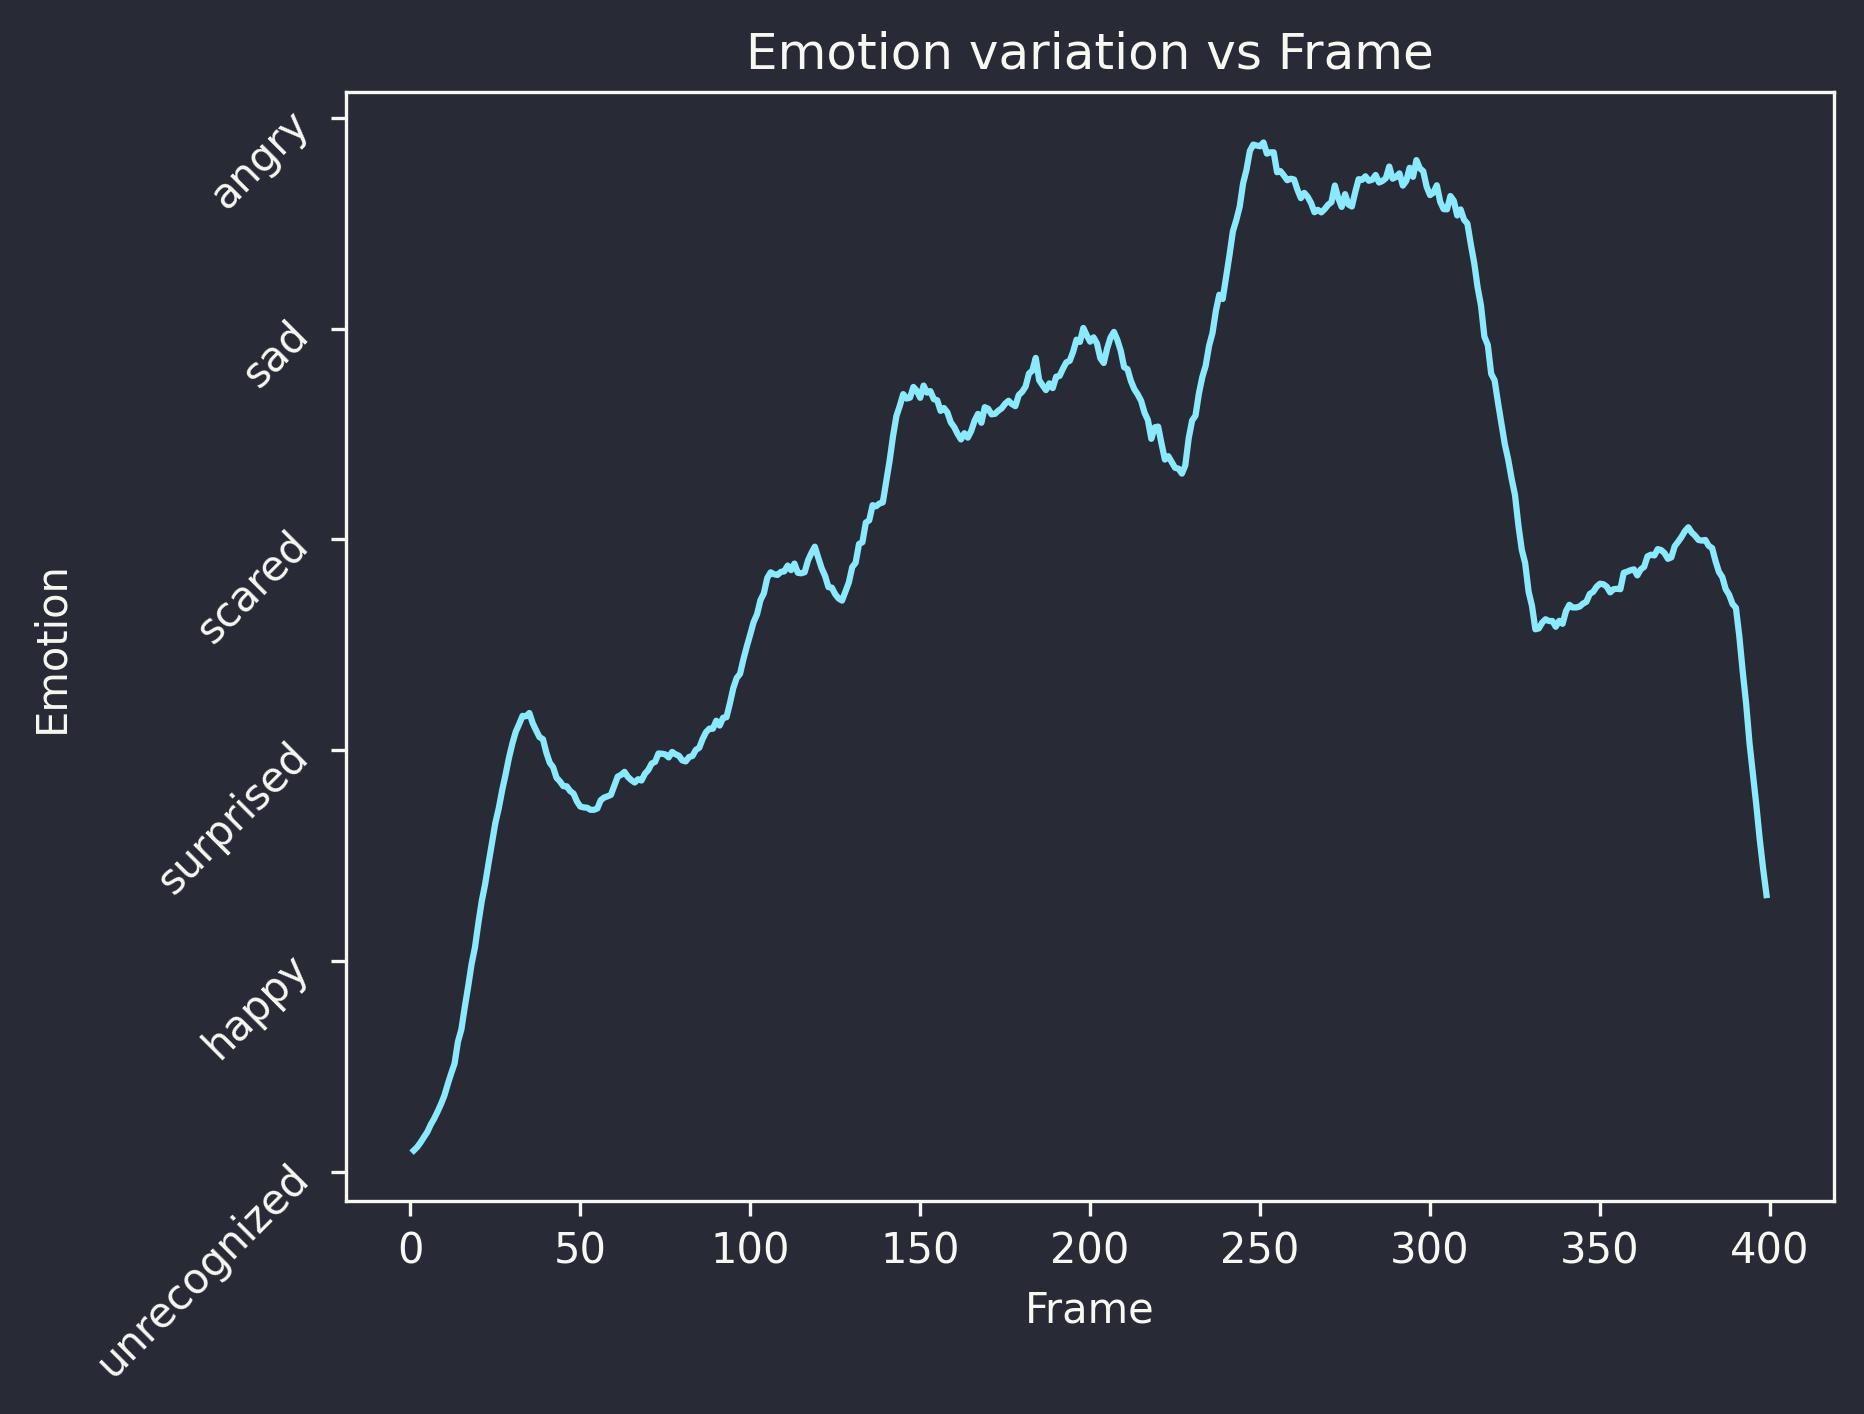
\includegraphics[height = 6cm]{resources/emotionvsframe.png}
         \caption{Emotion variation by frame of a sample.}\label{fig:emotionvsframe}
       \end{subfigure}
    \caption{Graphs for face and emotion detection performance.} \label{fig:emotionandtime}
    \end{figure}
  
Towards real-time: detecting face->crop->emotion detector if face is persistent 

Explanation about the performance evaluation procedure and results analysis.


\subsection{Style transfer}

-> switch style context if emotion is persistent.


\begin{figure}[ht]
    \centering
        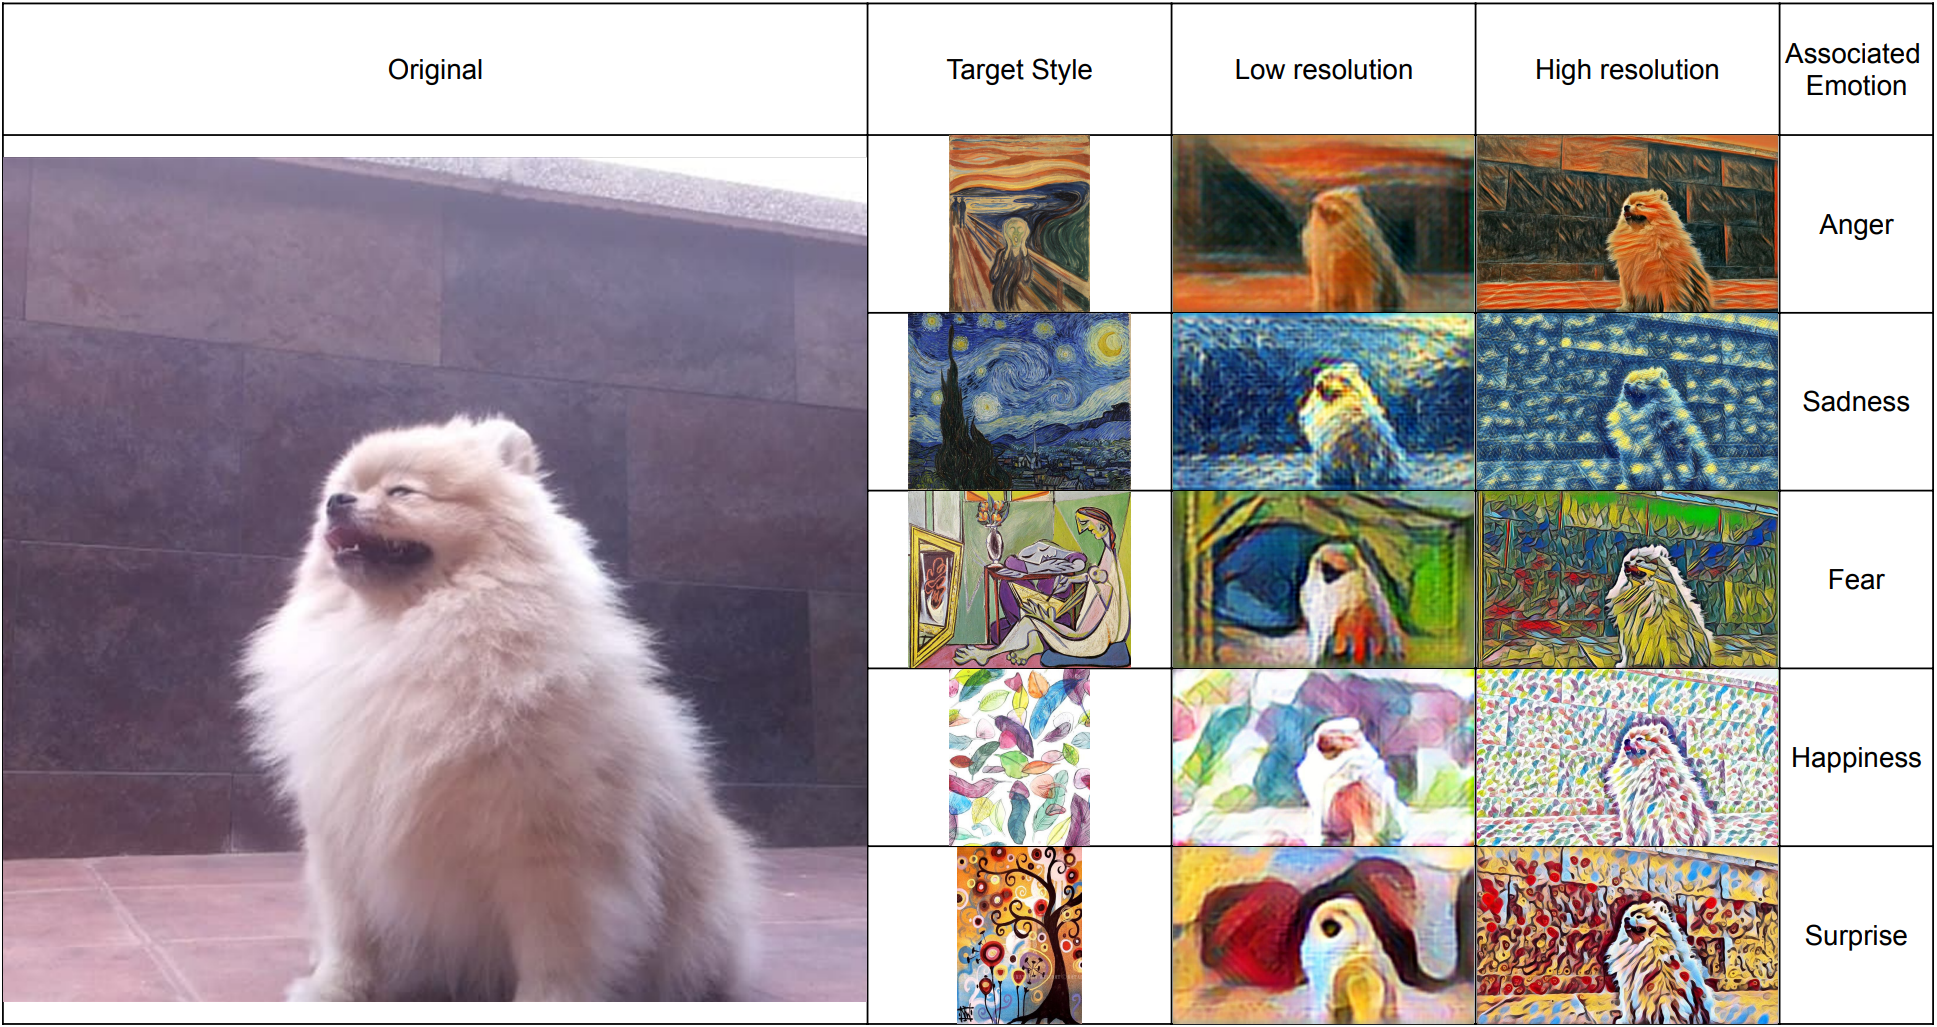
\includegraphics[width=\textwidth]{resources/styletransfer_emogrid.png}        
        \caption{Available style transfers for emotion context switching sample. From top to bottom: 
            \emph{The scream by Edvard Munch, 
            The Starry Night by Vincent Van Gogh, 
            La Musa (Mujer Leyendo) by Pablo Picasso, 
            Feathers b Kathryn Corlett, 
            June tree BY Natasha wescoat.
            }
    } \label{fig:style_grid}
\end{figure}


This train of thought proved to be flawed, as we minimally improved the speed of inference of the models, while taking a massive hit on image quality for style transfer.
